\documentclass[12pt]{article}
\usepackage{amsmath, amsthm, amssymb, amsfonts}
\usepackage{hyperref}
\usepackage{graphicx}
\usepackage{float}
\usepackage{xcolor}

\DeclareMathOperator*{\argmin}{argmin}

%opening
\title{Flat Norm on Graphs}
\author{Sandy Auttelet, Jared Brannan, Blake Cecil, Curtis Michels,\\
 Katrina Sabochick, Kevin Vixie }

\begin{document}

\maketitle

\begin{abstract}
In this paper we implement and test a method for computing the multiscale flat norm signature for characteristic functions over irregular grids in $\mathbb{R}^2$ and $\mathbb{R}^3$.
\end{abstract}

\tableofcontents

\section{Multiscale Flat Norm}

In 2005, Chan and Esedoglu introduced an edge preserving total variation regularization functional:

\begin{equation} \label{ce}
F_{CE}(u,f) = \int_\Omega |\nabla u| dx + \lambda \int_{\Omega} |u-f|dx
\end{equation}

\noindent  Where $\Omega$ is a domain on which we have greyscale data $f:\Omega \to \mathbb{R}$ we would like to denoise. Solving the associated minimization problem above we obtain:

\begin{align*}
u^* = \argmin_u F_{CE}(u,f)
\end{align*}

 \noindent Where $u^*: \Omega \rightarrow \Omega$ is the denoised greyscale approximation to the data $f$.
 
The strength of the denoising may be adjusted by the parameter $\lambda \in [0,\infty)$, a large value of $\lambda$ corresponds to enacting a stricter penalty for candidates $u$ that deviate too far from the original data and thus enforce less denoising. We henceforth refer to (\ref{ce}) as the $L^1$TV functional.

It was recognized in \cite{Morgan_2007} by Simon Morgan and Kevin Vixie that the $L^1$TV functional was both a special case of and an extension of the flat norm in geometric measure theory (GMT). The work done in \cite{shapes, hu_median, ibrahim_simplicial, fn_decomp} explore the implications of this. These tools have subsequently found applications in chemistry \cite{flat_norm_chemistry_fingers} and engineering \cite{meyur2023structural, aouada2009squigraphs}.


\section{Discrete Implementations}

Let $\chi_E$ be the characteristic function of $E$, with $\chi_E(x) = 1$ if $x \in E$ and $0$ otherwise. Then $u$ may be taken to be of this form, and the $L^1$TV functional in (\ref{ce}) reduces to:

\begin{align*}
F_{CE}(\Sigma,\Omega) &= \text{Per}(\Sigma) + \lambda|\Sigma \Delta \Omega|
\end{align*}

 \noindent where $\Sigma$ is the support of $u = \chi_\Sigma$, Per($\Sigma$) is the perimeter of $\Sigma$, and $\Sigma \Delta \Omega$ is the symmetric difference between $\Sigma$ and the support $\Omega$ of the data $f = \chi_\Omega$ (see \cite{ce} for the details). 

The flat norm with scale $\lambda$ of an oriented $1$-dimensional set $T$ is given by:

\begin{equation} \label{fn}
\mathbb{F}_\lambda(T) = \min_S \{V_1(T-\partial S) + \lambda V_2(S)\}
\end{equation}

 \noindent  Where $V_1$ is 1-dimensional volume (length), $V_2$ is 2-dimensional volume (area) and $S$ varies over oriented $2$-dimensional regions. We refer to the pair of the 1D and 2D sets $\{T,S^*\}$ as the flat norm decomposition, where $S^*$ is the minimizer of $(\ref{fn})$. In \cite{Morgan_2007} Morgan and Vixie established for $\Omega \subseteq \mathbb{R}^n$,

\begin{equation}
\mathbb{F}_\lambda(\partial^* \Omega) = \min_{\Sigma} F_{CE}(\Sigma,\Omega)
\end{equation}

 \noindent Where $\partial^*$ denotes the reduced boundary of $\Omega$ (up to a set of $H^{n-1}$ measure zero $\partial^* \Omega$ is equal to the measure theoretic boundary of $\Omega$.)

Practically, Vixie and Morgan \cite{shapes} tells us that we can use any method that solves the Chan-Esedoglu problem to compute the flatnorm for co-dimension 1 boundaries. Subsequently they used the graph cut method introduced in \cite{kolmogorov}. Additional methods based on simplicial complexes have been developed since that  extend the multiscale flat norm to inputs that are not necessarily boundaries \cite{ibrahim_simplicial}.

Applied to images, this is realized by representing each pixel as a node on a rectangular grid which forms the working space. A characteristic function $\chi_\Omega$ is defined on the nodes which represents a black and white thresholded image. Graph edges are added between each node using the 16 distinct directions in image space. Each of these edges are weighted by minimizing gradient computation error on known linear functions. After, a virtual sink ($t$) and a virtual source node ($s$) are added. The source node is connected to every node in $\Omega$ and the sink to every node on the grid not in $\Omega$. 

With the correct setting of weights a cut of this graph has a capacity equal to $F_{CE}(\Sigma,\Omega)$. For $\Sigma$ treated as the set of nodes in the graph that are either (1) connected to the source by an edge not cut or (2) are connected ot the sink by an edge that is cut, any cut of the graph incurs a penalty equal to $F_{CE}(\Sigma,\Omega)$ Hence finding a cut with minimal capacity is the same as computing a discrete approximation to $F_{CE}(\Sigma,\Omega)$ and hence an approximation to the flat norm as well. 

\begin{figure}[H]
	\centering
	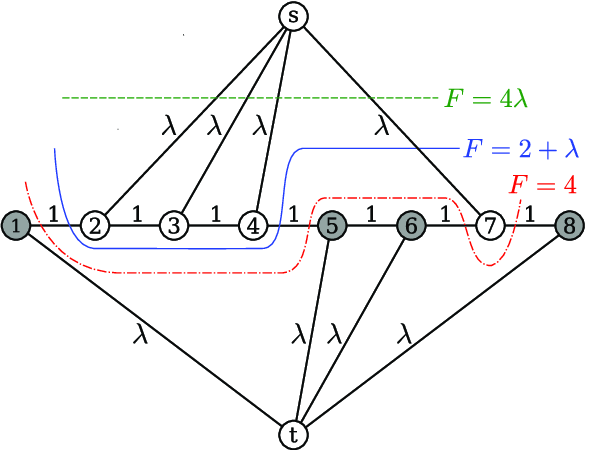
\includegraphics[scale=1]{graph-cut-for-a-1-dimensional-image.png}
	\caption{A discrete approximation to $F_{CE}(\Sigma,\Omega)$ using graph cuts from \cite{Morgan_2007}.}
\end{figure}

The vector of weights $w^*$ calculated in \cite{shapes} were chosen more specifically to approximate the linear function $g_\theta:\mathbb{R}^2 \to \mathbb{R}$ whose gradient is $\nabla g_\theta = (\cos \theta, \sin \theta)^T$ for all $\theta$:

\begin{equation} \label{oldmin}
w^* = \argmin_w \int_0^{2\pi} (h(w,\theta)-1)^2 d\theta
\end{equation}

With

\begin{align*}
h(w,\omega) &= \sum_{j=1}^4 w_1 |\nabla g_\theta \cdot v_j| + \sum_{j=5}^8 w_2 |\nabla g_\theta \cdot v_j| +  \sum_{j=9}^{16} w_3 |\nabla g_\theta \cdot v_j|
\end{align*}

Where $v_j, j= 1,...,16$ are the vectors from a fixed point in the grid to its 16 nearest neighbors, where three types of neighbor groupings are identified as below.

\begin{figure}[H]
\centering
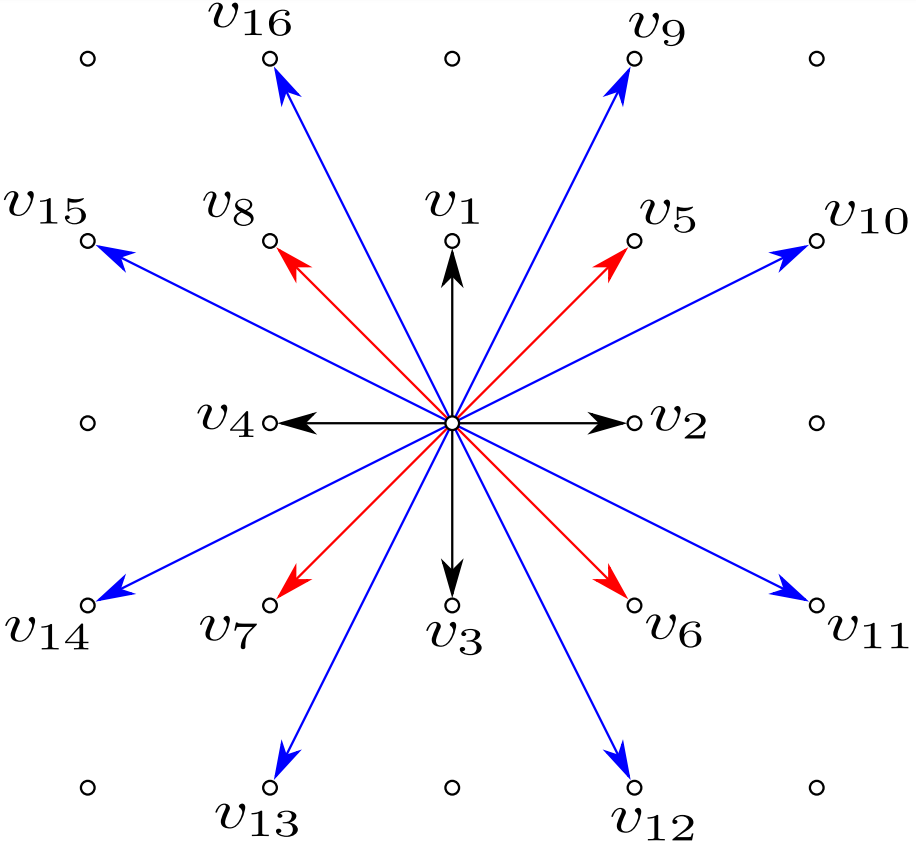
\includegraphics[scale=0.25]{Figure_2_Vixie_Paper.png}
\caption{16 vector neighborhood from \cite{shapes}.}
\end{figure}

Equation (\ref{oldmin}) was solved analytically to obtain weights $(w_1,w_2,w_3) \approx (0.1221,0.0476,0.0454)$. 


\section{Flat Norm on Arbitrary 2D and 3D Graphs}

In the present work, we extend the multiscale flat norm computation to arbitrary graphs embedded in $\mathbb{R}^n$ using the framework above, and provide code to calculate explicitly in $\mathbb{R}^2$ and $\mathbb{R}^3$.

Let $V = \{v_1,...,v_N\}$ be a set of vertices in $\mathbb{R}^n$ with a set of edges $E$ on $V$. Fix a particular vertex $v \in V$ with degree $D$ and associated edges  $\{u_i\}_{i=1}^D$. We provide a scheme for calculating the edge weights $\{w_i\}_{i=1}^D$ that recover the weights obtained in (\ref{oldmin}) in the case of a regular unit grid and extend to arbitrary irregular grids and connections. Our weights will be chosen to minimize the distance (in the $L^2$ sense) between the weighted sum of the edges and the length of the graident vector $\nu$ on $\partial B(0,1)$, the unit sphere at the origin:

\begin{align}
\mathcal{F}(w_1,w_2,...,w_D) &:= \int_{\partial B(0,1)} \left|\sum_{i=1}^D w_i |\langle \nu, u_i \rangle| - 1 \right|^2d\nu\\
&= \sum_{i=1}^D w_i^2C_1^i + 2 \sum_{i=1}^D \sum_{j=1}^{i-1} w_i w_j C_3^{ij} - 2 \sum_{i=1}^D w_i C_2^i + \alpha(n)
\end{align}

Where $\alpha(n) = \int_{\partial B(0,1)}d\nu$ is the measure of $\mathbb{S}^{n-1}$ in $\mathbb{R}^n$. 

\begin{align*}
C_1^i &:= \int_{\partial B(0,1)} |\langle \nu,u_i \rangle|^2 d\nu\\
C_2^i &:= \int_{\partial B(0,1)} |\langle \nu,u_i \rangle| d\nu\\
C_3^{ij} &:= \int_{\partial B(0,1)} |\langle \nu,u_i \rangle \langle \nu, u_j \rangle| d\nu
\end{align*}

The weights are found via the gradient:

\begin{align*}
	\frac{\partial \mathcal{F}}{\partial \omega_k}  &= 2 \omega_k C_1^k + 2 \sum_{m=1}^{D}\omega_{m}C_{3}^{km} - 2\omega_kC_3^{kk} - 2 C_2^k\\
\end{align*}

Which yields a linear system of $D$ equations in $D$ unknowns. We then solve the following system for a stationary point:

\begin{align*}
2 \omega_1 C_1^1 + 2 \sum_{m=2}^{D}\omega_{m}C_{3}^{1m}  - 2 C_2^1 &= 0\\
\vdots \hspace{20mm} & \\
2 \omega_D C_1^D + 2 \sum_{m=1}^{D-1}\omega_{m}C_{3}^{Dm} - 2 C_2^D &= 0\\
\end{align*}

In practice this is done using least squares. The Hessian of $\mathcal{F}$ is:

\begin{align*}
\frac{\partial^2 \mathcal{F}}{\partial \omega_k \partial \omega_\ell} &= \begin{cases}
2C_1^k & \text{ if } \ell = k\\
2C_3^{k\ell} & \text{ otherwise}
\end{cases}
\end{align*}

And by inspection we see that $\mathcal{F}$ is convex, thus any stationary point yields a global minima. 

Thus the problem reduces to calculation of $C_1^i$, $C_2^i$ and $C_3^{ij}$. We provide the following table of values:

\begin{figure}[H]
\centering
\begin{tabular}{|c|c|c|c|}
\hline
 &  2D  & 3D  \\
\hline
 $C_1^i$ & $\pi \| u_i \|^2$  & $\frac{4\pi}{3}\|u_i\|^2$   \\
\hline
 $C_2^i$ & $4\| u_i \|$  & $2\pi \|u_i\|$    \\
\hline
 $C_3^{ij}$ & Numerical  & Numerical    \\
\hline
\end{tabular}
\end{figure}

Solving this system produces a weight $w_i$ for each edge $u_i$ for the vertex $v$, in order to approximate the total variation integral in (5) we multiply each weight by the area of its associated Voronoi cell. With the weighted graph we can then apply the min-cut max-flow algorithm after connecting vertices to the virtual source and sink as previously described.

The overall runtime complexity of the algorithm is estimated as follows. For a graph with $V$ vertices of degree $D$, and $E$ edges, we estimate the run time to be
\begin{align}
	O(|V|\log|V| + |V||D|^3 + |V|^2|E|)
\end{align}
Where the first term comes from constructing a $k$-d tree, the second from solving the $D \times D$ weight system for each vertex and the final term comes from the choice of min cut max flow algorithm.  


\section{Tests}

\subsection{Implementation and Visualizations}

The flat norm decomposition may be calculated on a greyscale image by first choosing a threshold value, pixels with a darkness above the threshold are treated as pure black with a value of ``1", forming the set $\Omega$ and those below the threshold are treated as pure white and are assigned a ``0" thus not belonging to $\Omega$. Thus the image is converted to a characteristic function $\chi_\Omega$.

All coordinates are then put into a KD-Tree structure and connections are formed between the $k$ nearest Euclidean neighbors, forming an initial graph. In our experiments, $k = 8$ neighbors provide the best balance of accuracy and speed. We then assign weights to these edges by solving the minimization problem at each node. Virtual sinks and sources are added with weight $\lambda$ and then a preflow-push algorithm computes the minimum cut yielding $\Sigma^* = \min\limits_\Sigma F_{CE}(\Sigma,\Omega)$.

$\Sigma^*$ is a approximation to $\Omega$ with curvature bounded by $\lambda$. Thus if $\lambda$ is larger than the maximum curvature of $\Omega$, $\Sigma^* = \Omega$ and the original image is returned. For $\lambda$ smaller than this, high curvature features are excluded, yielding a increasingly ``smoothed" result, wherein the limit $\lambda \to 0$ the empty set is returned.

Figure 3 highlights that for $\lambda$ large we will be able to reconstruct the set exactly but as $\lambda$ becomes smaller, circles of radius $r$ with $r < \frac{2}{\lambda}$ will begin to disappear in the reconstruction.


\begin{figure}[H]
	\centering
	
\includegraphics[scale=0.4]{figures/circlesgraph.png}
	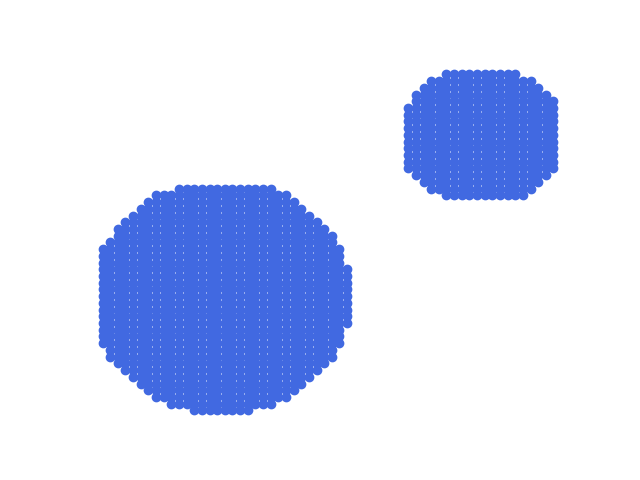
\includegraphics[scale=0.4]{figures/circlesdisappear.png}
	\caption{The flat norm reconstruction of the image, as lambda decreases higher curvature regions are removed.}
\end{figure}




\begin{figure}[H]
	\centering
	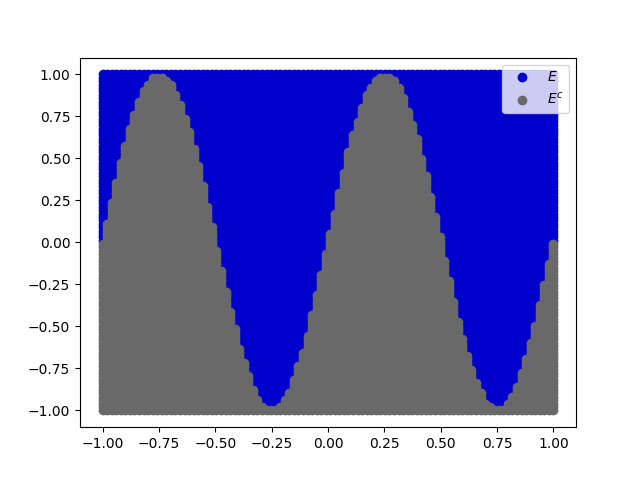
\includegraphics[scale=0.6]{figures/epigraph.png}
	\caption{The epigraph of a $\sin$ curve with the background grid in gray.}
\end{figure}

More insight can be gained by breaking down the sets in play for a particular image in further detail. Here we consider a set $E$ given by the epigraph of $f(x) = \sin(16\pi x)$. Let $\Sigma$ be the minimizer produced by approximating $E$ with the background grid labeled in grey for some $\lambda$. Fig 5 shows that regions of high curvature $\Sigma^C \cap E$ are removed from the solution and regions in the background grid but not in $E$ i.e. $\Sigma \cap E^C$ are also introduced to fill in regions of high curvature. The overall minimizer is then built out of both of these regions i.e. $\Sigma = (\Sigma \cap E) \cup (\Sigma \cap E^c)$.

\begin{figure}[H]
	\centering
	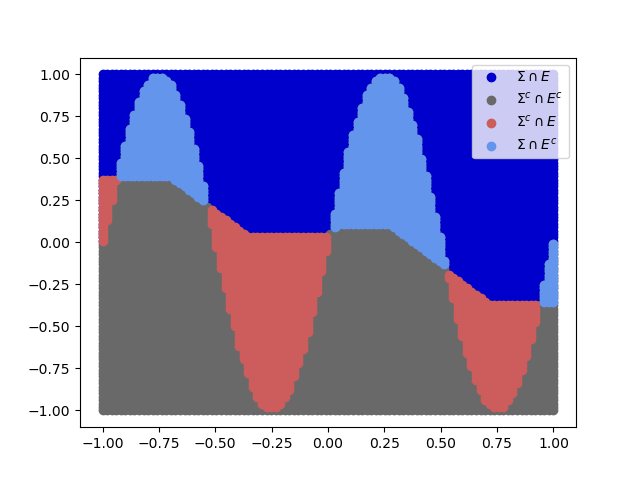
\includegraphics[scale=0.6]{figures/minimizer_detail.png}
	\caption{The flat norm reconstruction of the $\sin$ curve, regions of high curvature are removed or filled in.}
\end{figure}


\subsection{Perimeter Calculation}

Since weights are chosen according to the $F_CE(\Sigma,\Omega)$ functional one is able to recover the perimeter of $\Sigma$. This is achieved by summing over weights for edges that cross from $\Sigma$ into the background image $\Omega$. We do this in 2D and 3D for the circle and sphere respectively, and get the following approximations.

\begin{figure}[H]
	\centering
	\begin{tabular}{|c|c|c|c|}
		\hline
		&  Grid Size & Perimeter Estimate Relative Error  \\
		\hline
		$\mathbb{S}^1$ & 30x30 &  2.6\%  \\
		\hline
		$\mathbb{S}^2$ & TBD & TBD    \\
		\hline
	\end{tabular}
	\caption{Estimates from the perimeter term for the volume of spheres.}
\end{figure}

For the graph defining the epigraph, this perimeter term gives the arc length of the graph over its domain. We estimate the arclength of $x^2$ and the functions $f_a(x) = \sin(2\pi ax)$ for several choices of $a$. The accuracy of the perimeter estimation becomes poor as frequency becomes higher, indicating a relationship between curvature and the accuracy of the flat norm approximation.

\begin{figure}[H]
	\centering
	\begin{tabular}{|c|c|c|c|}
		\hline
		function & Arc Length Estimate Relative Error  \\
		\hline
		$x^2$   &  0.22\%  \\
		\hline
		$f_{2}(x)$  & 2.42\%    \\
		\hline
		$f_{4}(x)$  & 4.62\%    \\
		\hline
		$f_{8}(x)$  & 8.45\%    \\
		\hline
		$f_{16}(x)$  & 20.41\%    \\
		\hline
	\end{tabular}
	\caption{Estimates of arclength with 100x100 grid and 8 NN approximation.}
\end{figure}

\section{Edge Cases}

A limitation of the current approach is that for sets $\Omega$ sufficiently close to the boundary of the image pathological behavior occurs.



\bibliographystyle{plain} % We choose the "plain" reference style
\bibliography{refs} % Entries are in the refs.bib file

\end{document}
